\documentclass[11pt,preprint, authoryear]{elsarticle}

\usepackage{lmodern}
%%%% My spacing
\usepackage{setspace}
\setstretch{1.5}
\DeclareMathSizes{12}{14}{10}{10}

% Wrap around which gives all figures included the [H] command, or places it "here". This can be tedious to code in Rmarkdown.
\usepackage{float}
\let\origfigure\figure
\let\endorigfigure\endfigure
\renewenvironment{figure}[1][2] {
    \expandafter\origfigure\expandafter[H]
} {
    \endorigfigure
}

\let\origtable\table
\let\endorigtable\endtable
\renewenvironment{table}[1][2] {
    \expandafter\origtable\expandafter[H]
} {
    \endorigtable
}


\usepackage{ifxetex,ifluatex}
\usepackage{fixltx2e} % provides \textsubscript
\ifnum 0\ifxetex 1\fi\ifluatex 1\fi=0 % if pdftex
  \usepackage[T1]{fontenc}
  \usepackage[utf8]{inputenc}
\else % if luatex or xelatex
  \ifxetex
    \usepackage{mathspec}
    \usepackage{xltxtra,xunicode}
  \else
    \usepackage{fontspec}
  \fi
  \defaultfontfeatures{Mapping=tex-text,Scale=MatchLowercase}
  \newcommand{\euro}{€}
\fi

\usepackage{amssymb, amsmath, amsthm, amsfonts}

\def\bibsection{\section*{References}} %%% Make "References" appear before bibliography


\usepackage[round]{natbib}

\usepackage{longtable}
\usepackage[margin=2.3cm,bottom=2cm,top=2.5cm, includefoot]{geometry}
\usepackage{fancyhdr}
\usepackage[bottom, hang, flushmargin]{footmisc}
\usepackage{graphicx}
\numberwithin{equation}{section}
\numberwithin{figure}{section}
\numberwithin{table}{section}
\setlength{\parindent}{0cm}
\setlength{\parskip}{1.3ex plus 0.5ex minus 0.3ex}
\usepackage{textcomp}
\renewcommand{\headrulewidth}{0.2pt}
\renewcommand{\footrulewidth}{0.3pt}

\usepackage{array}
\newcolumntype{x}[1]{>{\centering\arraybackslash\hspace{0pt}}p{#1}}

%%%%  Remove the "preprint submitted to" part. Don't worry about this either, it just looks better without it:
\makeatletter
\def\ps@pprintTitle{%
  \let\@oddhead\@empty
  \let\@evenhead\@empty
  \let\@oddfoot\@empty
  \let\@evenfoot\@oddfoot
}
\makeatother

 \def\tightlist{} % This allows for subbullets!

\usepackage{hyperref}
\hypersetup{breaklinks=true,
            bookmarks=true,
            colorlinks=true,
            citecolor=blue,
            urlcolor=blue,
            linkcolor=blue,
            pdfborder={0 0 0}}


% The following packages allow huxtable to work:
\usepackage{siunitx}
\usepackage{multirow}
\usepackage{hhline}
\usepackage{calc}
\usepackage{tabularx}
\usepackage{booktabs}
\usepackage{caption}


\newenvironment{columns}[1][]{}{}

\newenvironment{column}[1]{\begin{minipage}{#1}\ignorespaces}{%
\end{minipage}
\ifhmode\unskip\fi
\aftergroup\useignorespacesandallpars}

\def\useignorespacesandallpars#1\ignorespaces\fi{%
#1\fi\ignorespacesandallpars}

\makeatletter
\def\ignorespacesandallpars{%
  \@ifnextchar\par
    {\expandafter\ignorespacesandallpars\@gobble}%
    {}%
}
\makeatother

\newenvironment{CSLReferences}[2]{%
}

\urlstyle{same}  % don't use monospace font for urls
\setlength{\parindent}{0pt}
\setlength{\parskip}{6pt plus 2pt minus 1pt}
\setlength{\emergencystretch}{3em}  % prevent overfull lines
\setcounter{secnumdepth}{5}

%%% Use protect on footnotes to avoid problems with footnotes in titles
\let\rmarkdownfootnote\footnote%
\def\footnote{\protect\rmarkdownfootnote}
\IfFileExists{upquote.sty}{\usepackage{upquote}}{}

%%% Include extra packages specified by user

%%% Hard setting column skips for reports - this ensures greater consistency and control over the length settings in the document.
%% page layout
%% paragraphs
\setlength{\baselineskip}{12pt plus 0pt minus 0pt}
\setlength{\parskip}{12pt plus 0pt minus 0pt}
\setlength{\parindent}{0pt plus 0pt minus 0pt}
%% floats
\setlength{\floatsep}{12pt plus 0 pt minus 0pt}
\setlength{\textfloatsep}{20pt plus 0pt minus 0pt}
\setlength{\intextsep}{14pt plus 0pt minus 0pt}
\setlength{\dbltextfloatsep}{20pt plus 0pt minus 0pt}
\setlength{\dblfloatsep}{14pt plus 0pt minus 0pt}
%% maths
\setlength{\abovedisplayskip}{12pt plus 0pt minus 0pt}
\setlength{\belowdisplayskip}{12pt plus 0pt minus 0pt}
%% lists
\setlength{\topsep}{10pt plus 0pt minus 0pt}
\setlength{\partopsep}{3pt plus 0pt minus 0pt}
\setlength{\itemsep}{5pt plus 0pt minus 0pt}
\setlength{\labelsep}{8mm plus 0mm minus 0mm}
\setlength{\parsep}{\the\parskip}
\setlength{\listparindent}{\the\parindent}
%% verbatim
\setlength{\fboxsep}{5pt plus 0pt minus 0pt}



\begin{document}



\begin{frontmatter}  %

\title{Russia-Ukraine Conflict: Insights for an Australian news desk}

% Set to FALSE if wanting to remove title (for submission)




\author[Add1]{Angela Euston-Brown\footnote{\textbf{Contributions:}
  \newline \emph{The student would like to thank the Ukraine Support
  Tracker for the data and Nico Katzke for the skills.}}}
\ead{28784618@sun.ac.za}





\address[Add1]{Stellenbosch University, Stellenbosch, South Africa}

\cortext[cor]{Corresponding author: Angela Euston-Brown\footnote{\textbf{Contributions:}
  \newline \emph{The student would like to thank the Ukraine Support
  Tracker for the data and Nico Katzke for the skills.}}}

\begin{abstract}
\small{
The Russia-Ukraine conflict has been on-going since 2014, with the
conflict escalating on the 24 February 2022. This document explores
which countries have been giving to the Ukrainian cause, since 2022, and
specifically explores whether the EU countries have been contributing
enough. The insights are summarised as bullet points for the Australian
news desk segment ``From Russia With No Love''. These findings form the
solution for Question 3 of the datascience exam.
}
\end{abstract}

\vspace{1cm}





\vspace{0.5cm}

\end{frontmatter}

\setcounter{footnote}{0}



%________________________
% Header and Footers
%%%%%%%%%%%%%%%%%%%%%%%%%%%%%%%%%
\pagestyle{fancy}
\chead{}
\rhead{}
\lfoot{}
\rfoot{\footnotesize Page \thepage}
\lhead{}
%\rfoot{\footnotesize Page \thepage } % "e.g. Page 2"
\cfoot{}

%\setlength\headheight{30pt}
%%%%%%%%%%%%%%%%%%%%%%%%%%%%%%%%%
%________________________

\headsep 35pt % So that header does not go over title




\hypertarget{introduction}{%
\section{\texorpdfstring{Introduction
\label{Introduction}}{Introduction }}\label{introduction}}

The Russia-Ukraine conflict has been on-going since 2014, with the
conflict escalating on the 24 February 2022. This document explores
which countries have been giving to the Ukrainian cause, since 2022. The
insights are summarised as bullet points for the Australian news desk
segment ``From Russia With No Love''.

It is important to note that allocations, in our understanding, refer to
sums of money allocated to a cause within a country's budget, while
commitments are pledges to allocate money to a cause. Thus, many
countries may commit to aid in the war effort, but never actually
allocate the contribution to said cause. This will be explored further
in the graphics below.

\hypertarget{are-the-eu-doing-enough}{%
\section{\texorpdfstring{Are the EU doing enough?
\label{EU}}{Are the EU doing enough? }}\label{are-the-eu-doing-enough}}

\textbackslash label\{Figure1\} below shows the sum of total allocated
aid and committed aid to Ukraine by donor group, namely the US, all EU
countries, and all other countries in the dataset.

\begin{itemize}
\item
  The plot shows that the EU have allocated less than non-EU countries,
  despite having 27 member states compared to only 12 (13 including the
  US) non-EU countries.
\item
  The plot further shows a large gap in the total commitments compared
  to the total allocations toward the war effort, particularly amongst
  EU nations.
\item
  The US is shown separately, as the country alone has committed more to
  the Ukrainian war effort than all other non-EU countries, as well as
  all EU countries. However, it is interesting to see that the US have
  yet to allocate any funds to the cause. Perhaps the EU aren't doing so
  badly after all.
\end{itemize}

\begin{figure}[H]

{\centering 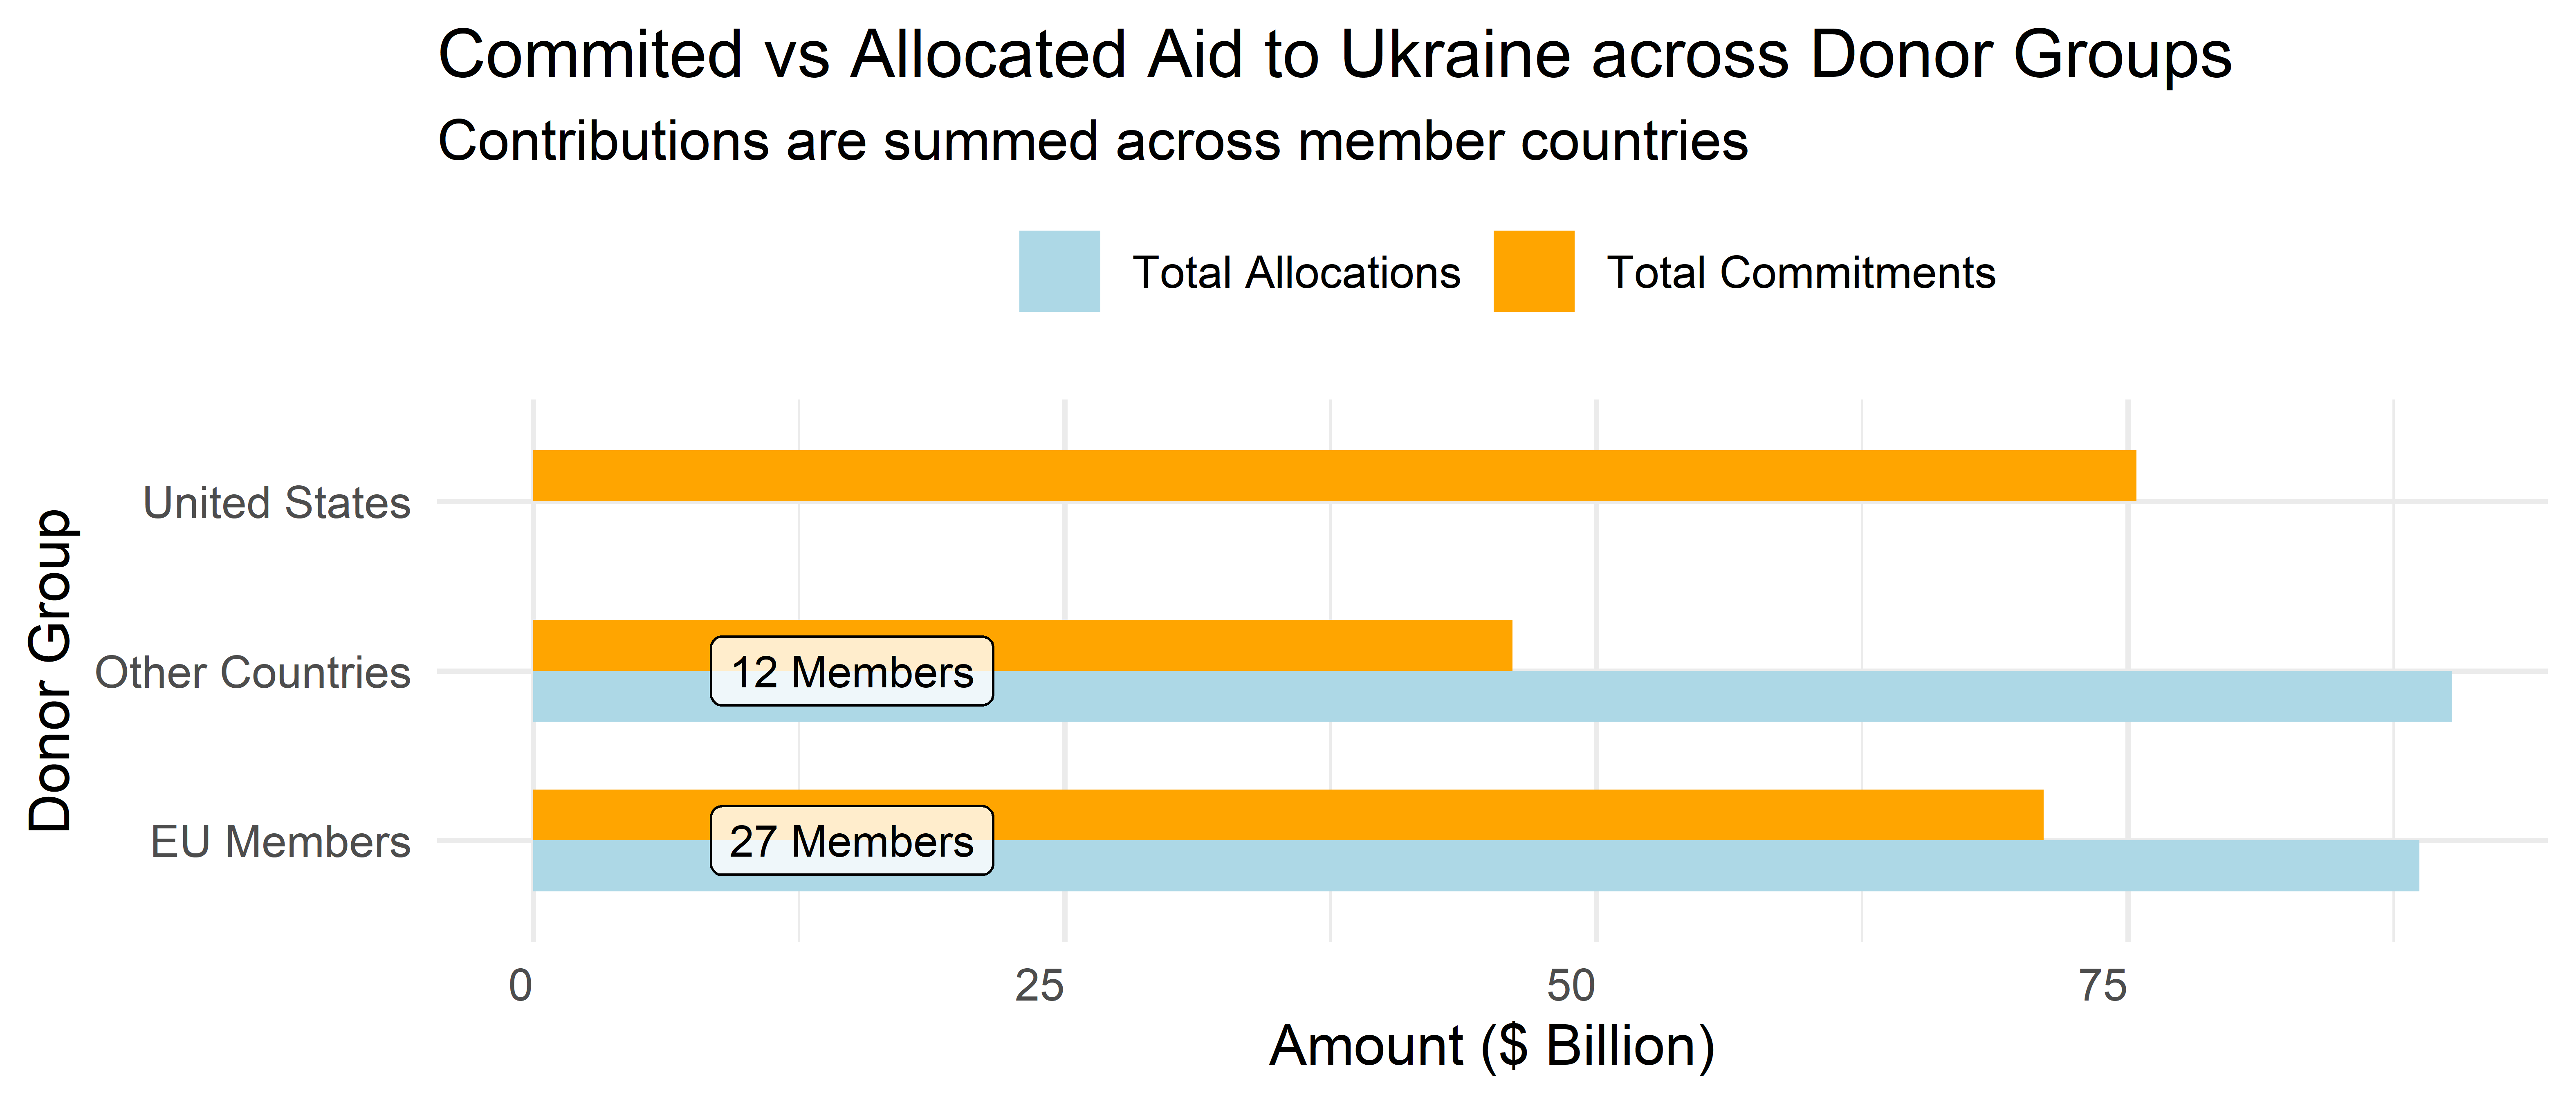
\includegraphics{Question_3_files/figure-latex/Figure1-1} 

}

\caption{EU Allocations \label{Figure1}}\label{fig:Figure1}
\end{figure}

\hypertarget{which-countries-are-pulling-their-weight}{%
\section{\texorpdfstring{Which countries are pulling their weight?
\label{vsGDP}}{Which countries are pulling their weight? }}\label{which-countries-are-pulling-their-weight}}

The figure produced below compares each country in the dataset's total
allocations and commitments as a percentage of their GDP, allowing us to
illustrate which countries are perhaps pulling more weight than others
based on their economic capacity.

The plot shows several interesting dynamics: * Countries are committing
between 0-3\% of their GDP, and this does not always lead to allocating
funds. * 4 EU countries are allocating considerably large proportions of
their GDP, most notably with Estonia allocating over 75\% of their GDP
to the cause. This sheds light on the economically small countries hopes
for Ukraine to win the war. * In terms of allocation, the UK have made
the largest total allocations as a percent of their GDP out of the
non-EU states. While Normay have the largest total commitments as a
percent of their GDP. * Despite allocating over 25\% of their GDP to the
cause, Malta have committed very little.

Ultimately, the figure emphasises that there are several small EU
countries that are doing a lot to stem the tide of the war despite their
own small economies.

\begin{figure}[H]

{\centering 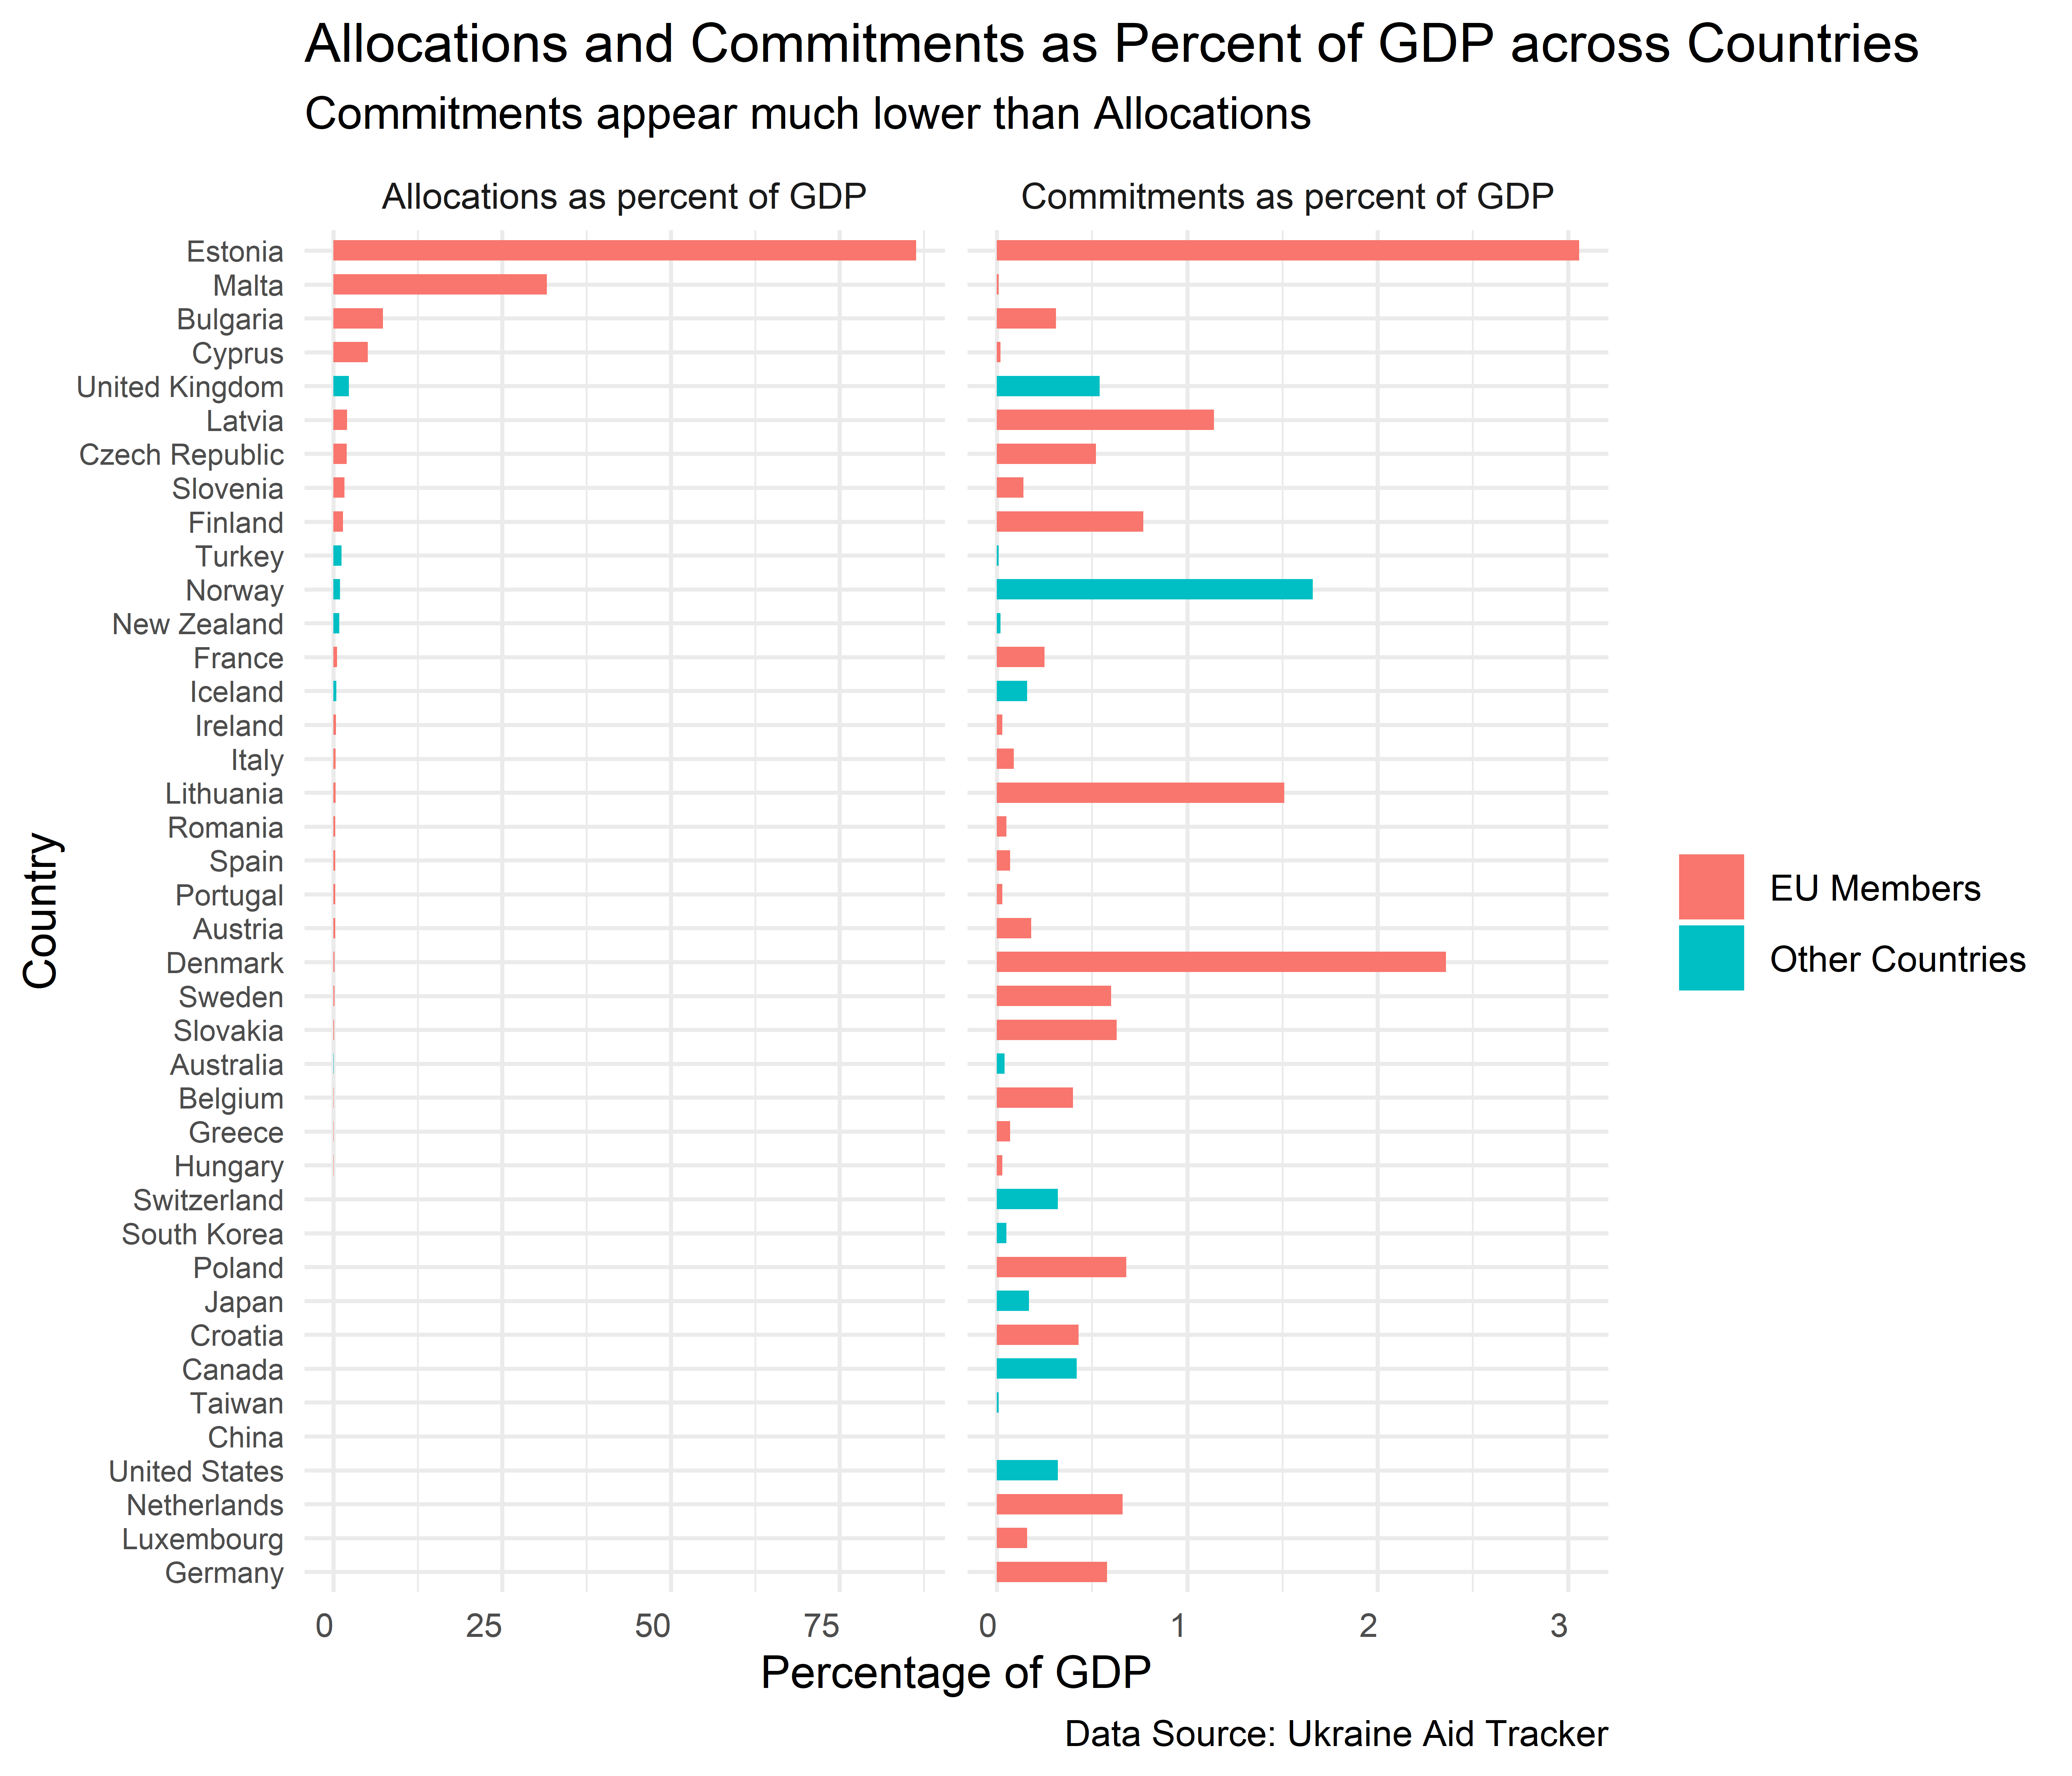
\includegraphics{Question_3_files/figure-latex/Figure2-1} 

}

\caption{Percent GDP \label{Figure2}}\label{fig:Figure2}
\end{figure}

\hypertarget{an-extra-detail-what-type-of-assistance-dominates-the-eus-war-aid}{%
\section{\texorpdfstring{An extra detail: What type of assistance
dominates the EU's war aid?
\label{aid_type}}{An extra detail: What type of assistance dominates the EU's war aid? }}\label{an-extra-detail-what-type-of-assistance-dominates-the-eus-war-aid}}

The third and last figure provides a little more information for those
curious viewers. The bar plot presents the total allocations of EU and
non-EU states, broken down into the different types of assistance.

\begin{itemize}
\item
  The plot shows that the EU offer more financial assistance to the war
  effort than other countries.
\item
  In comparison, non-EU countries predominantly offer military
  assistance.
\item
  Total commitments are also indicated with a black dot, to reiterate
  the differences between donor groups' commitments and allocations.
\end{itemize}

\begin{figure}[H]

{\centering 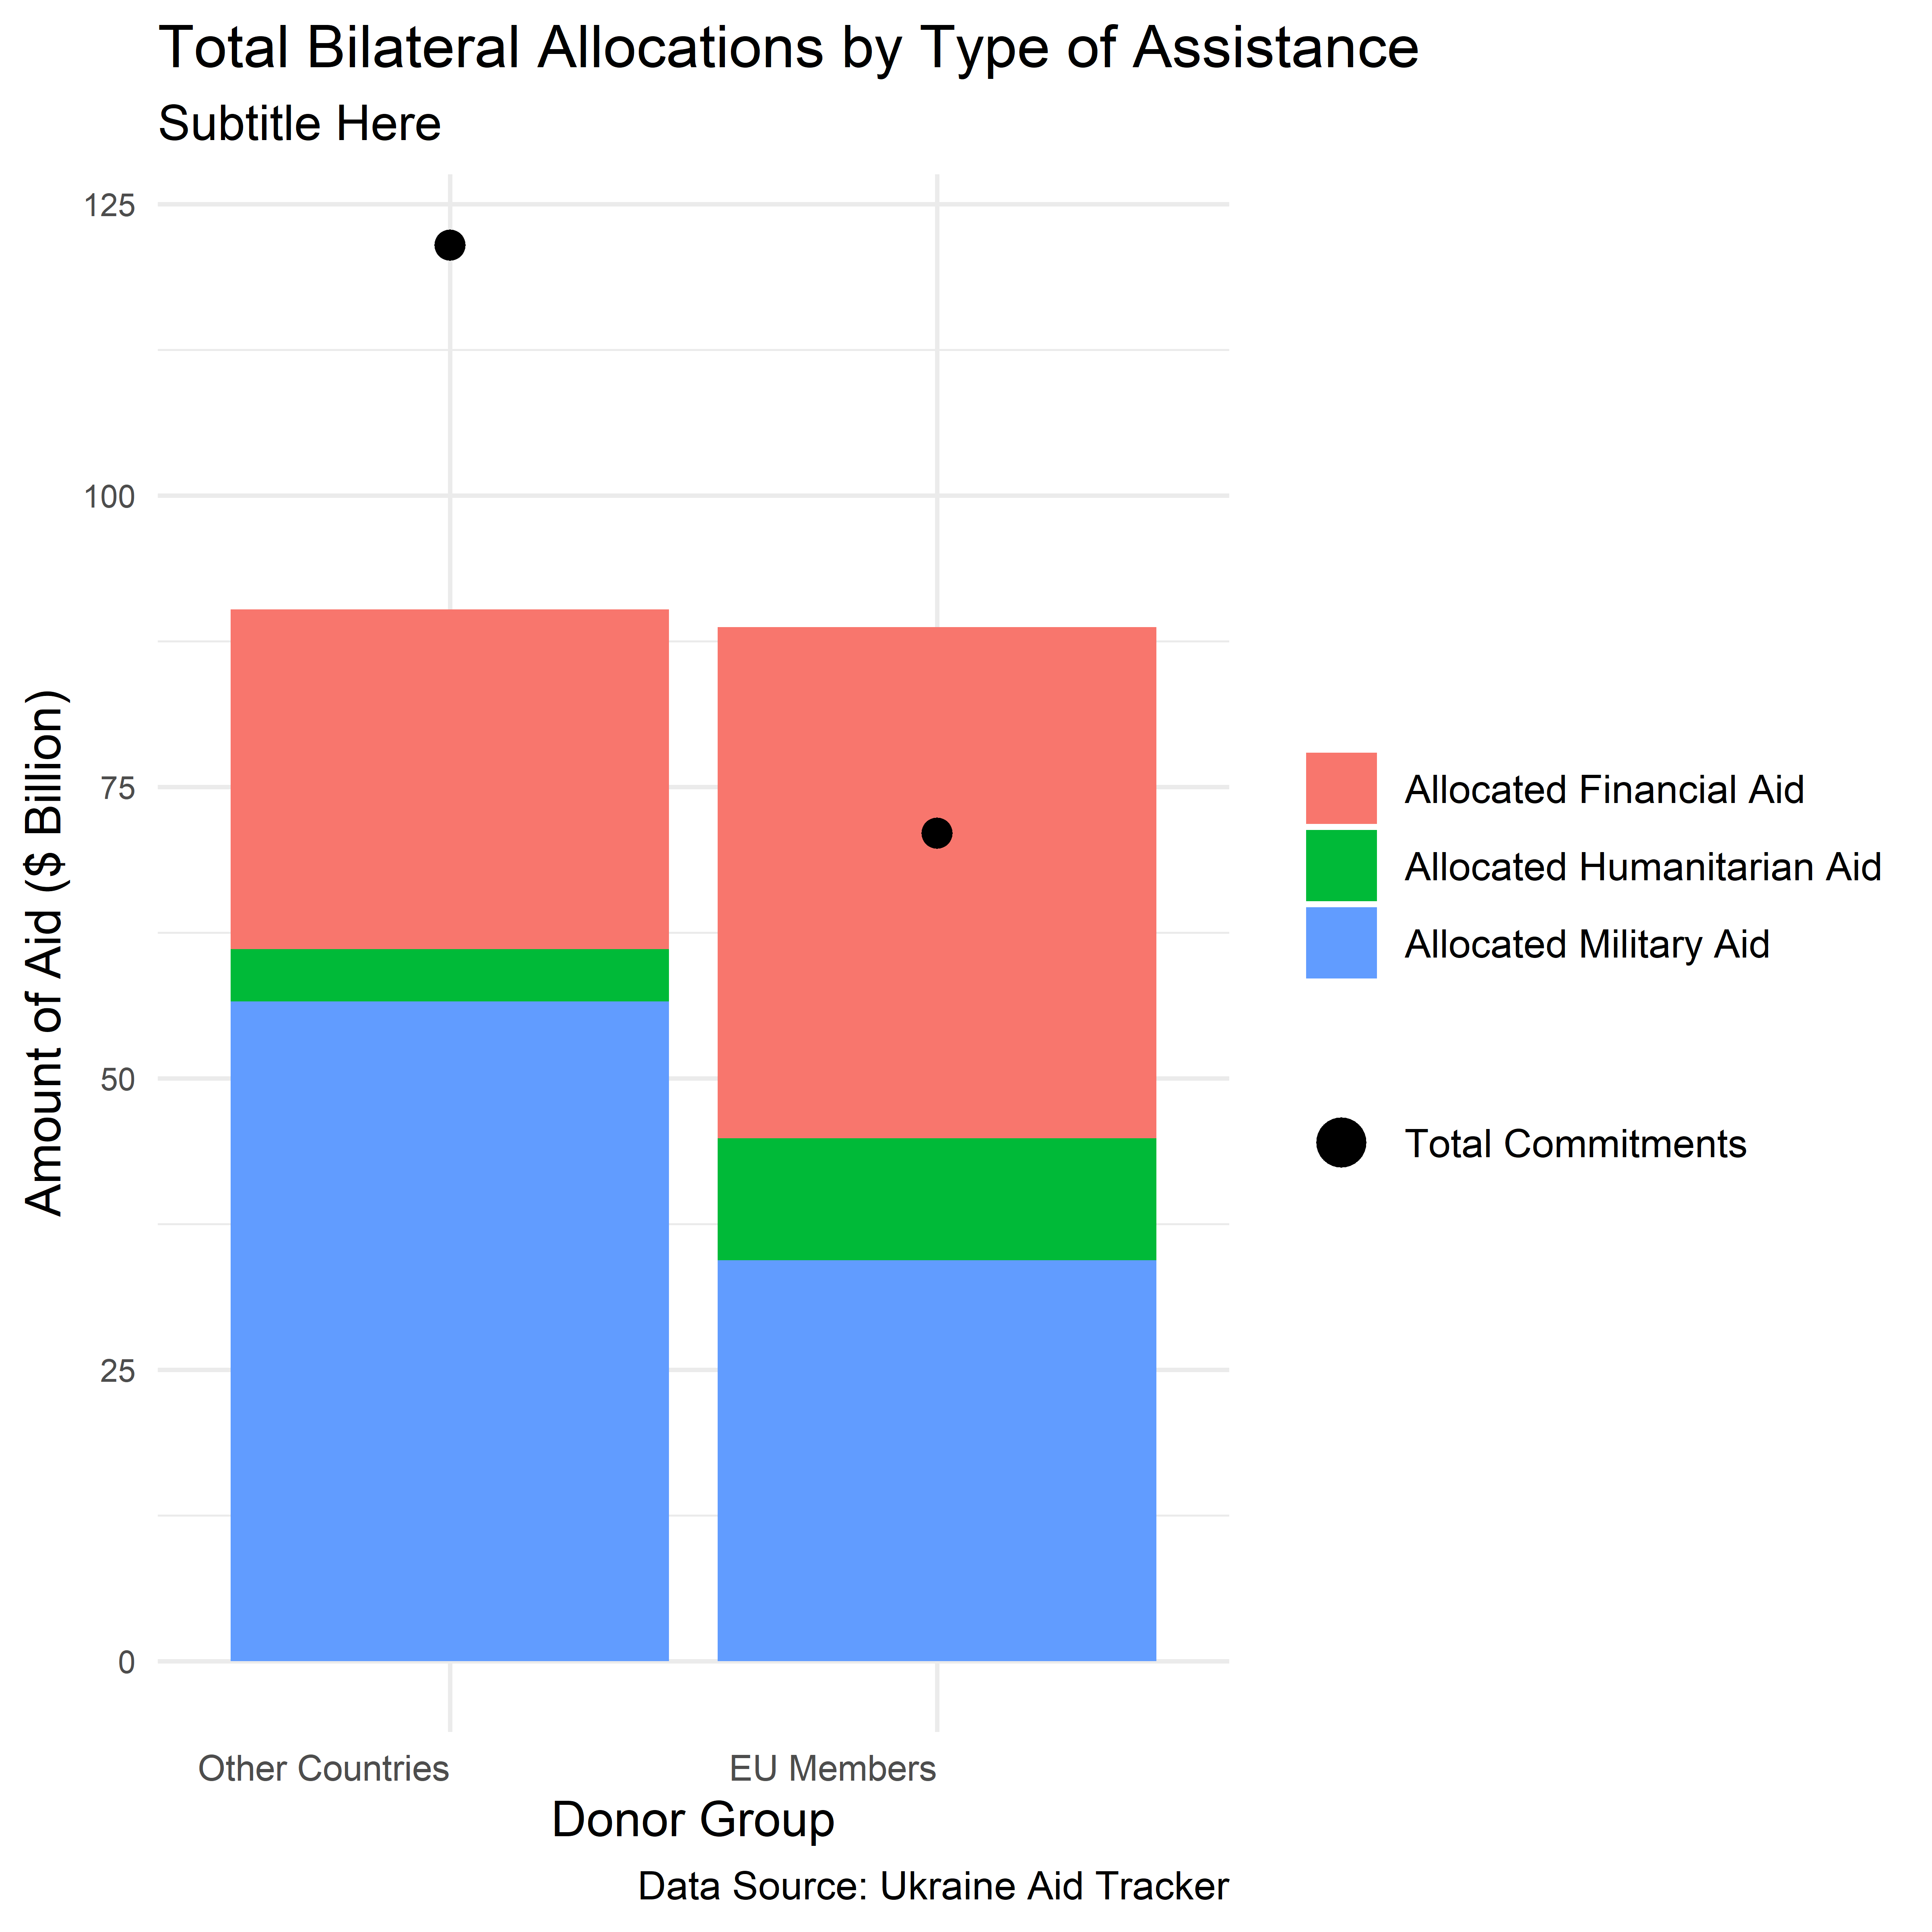
\includegraphics{Question_3_files/figure-latex/Figure3-1} 

}

\caption{Aid Type \label{Figure3}}\label{fig:Figure3}
\end{figure}

\hypertarget{summary-for-interpretation-on-air}{%
\section{Summary for Interpretation on
Air}\label{summary-for-interpretation-on-air}}

\begin{itemize}
\item
  The EU have not allocated more to the war effort than other countries,
  despite having more member states.
\item
  Small EU countries are contributing considerable proportions of their
  GDP to stem the tide of the Ukraine-Russia war.
\item
  The EU offer almost equal quantities of military and financial aid,
  but appear to be offering comparatively more financial aid than other
  non-EU countries.
\end{itemize}

This pdf was put together using
Texevier(\protect\hyperlink{ref-Texevier}{Katzke, 2017}).

\newpage

\hypertarget{references}{%
\section*{References}\label{references}}
\addcontentsline{toc}{section}{References}

\hypertarget{refs}{}
\begin{CSLReferences}{1}{0}
\leavevmode\vadjust pre{\hypertarget{ref-Texevier}{}}%
Katzke, N.F. 2017. \emph{{Texevier}: {P}ackage to create elsevier
templates for rmarkdown}. Stellenbosch, South Africa: Bureau for
Economic Research.

\end{CSLReferences}

\bibliography{Tex/ref}





\end{document}
